%%%%%%%%%%%%%%%%%%%%%%%%%%%%%%%%%%%%%%%%%%%%%%%%%%%%%%%%%%%%%%%%%%%%%
%
%  This is a sample LaTeX input file for your contribution to
%  the PHYSOR2020 topical meeting.
%
%  Please use it as a template for your full paper
%    Accompanying/related file(s) include:
%       1. Document class/format file: physor2020.cls
%       2. Sample Postscript Figure:   figure.pdf
%       3. A PDF file showing the desired appearance: physor2020_template.pdf
%       4. cites.sty and citesort.sty that might be needed by some users
%    Direct questions about these files to: rcarlos.lope@gmail.com
%											armando.gomez@inin.gob.mx
%
%    Notes:
%      (1) You can use the "dvips" utility to convert .dvi
%          files to PostScript.  Then, use either Acrobat
%          Distiller or "ps2pdf" to convert to PDF format.
%      (2) Different versions of LaTeX have been observed to
%          shift the page down, causing improper margins.
%          If this occurs, adjust the "topmargin" value in the
%          physor2020.cls file to achieve the proper margins.
%
%%%%%%%%%%%%%%%%%%%%%%%%%%%%%%%%%%%%%%%%%%%%%%%%%%%%%%%%%%%%%%%%%%%%%


%%%%%%%%%%%%%%%%%%%%%%%%%%%%%%%%%%%%%%%%%%%%%%%%%%%%%%%%%%%%%%%%%%%%%
\documentclass[letterpaper]{physor2020}
%
%  various packages that you may wish to activate for usage
\usepackage{tabls}
\usepackage{cites}
\usepackage{epsf}
\usepackage{appendix}
\usepackage{ragged2e}
\usepackage[top=1in, bottom=1.in, left=1.in, right=1.in]{geometry}
\usepackage{enumitem}
\setlist[itemize]{leftmargin=*}
\usepackage{caption}
\captionsetup{width=1.0\textwidth,font={bf,normalsize},%
              skip=0.3cm,within=none,justification=centering}
\usepackage{bm}
\usepackage{tikz}
\usepackage{xfrac}
\usepackage{units}

% Daniele: I commented this part because it was not present in the original
% conference template.
% % for quotes
% \usepackage[english]{babel}
% \usepackage[autostyle, english = american]{csquotes}
% \MakeOuterQuote{"}
%
\newcommand{\eq}[1]{Eq.~(\ref{#1})}
\newcommand{\eqnolabel}[1]{(\ref{#1})}
\newcommand{\eqs}[1]{Eqs.~(\ref{#1})}
\newcommand{\eqsthru}[2]{Eqs.~(\ref{#1})--(\ref{#2})}
\newcommand{\eqsand}[2]{Eqs.~(\ref{#1}) and (\ref{#2})}
\newcommand{\tbl}[1]{Table~\ref{#1}}
\newcommand{\tblnolabel}[1]{\ref{#1}}
\newcommand{\tbls}[1]{Tables~\ref{#1}}
\newcommand{\tblsthru}[2]{Tables~\ref{#1}--\ref{#2}}
\newcommand{\tblsand}[2]{Tables~\ref{#1} and \ref{#2}}
\newcommand{\fig}[1]{Fig.~\ref{#1}}
\newcommand{\fignolabel}[1]{\ref{#1}}
\newcommand{\figs}[1]{Figs.~\ref{#1}}
\newcommand{\figsthru}[2]{Figs.~\ref{#1}--\ref{#2}}
\newcommand{\figsand}[2]{Figs.~\ref{#1} and \ref{#2}}
\newcommand{\sxn}[1]{Section~\ref{#1}}
%
% \newcommand{\tsup}[1]{\textsuperscript{#1}}
% \newcommand{\tsub}[1]{\textsubscript{#1}}
%
\newcommand{\keff}{{\ensuremath{k_{\textrm{\scriptsize{eff}}}}}}
\newcommand{\kinf}{\ensuremath{k_{\textrm{\scriptsize{$\infty$}}}}}
\newcommand{\beff}{\ensuremath{\beta_{\textrm{eff}}}}
\newcommand{\eg}{e.g.,}
\newcommand{\ie}{i.e.,}
\newcommand{\OO}{\ensuremath{\hat{\bm{\Omega}}}}
\newcommand{\rr}{\ensuremath{\bm{r}}}
\newcommand{\bnabla}{\ensuremath{\bm{\nabla}}}
\newcommand{\rE}{\ensuremath{(\rr,E)}}

\newcommand{\ftr}{\ensuremath{\phi_{\textrm{\scriptsize{tr}}}}}
\newcommand{\jtr}{\ensuremath{\bm{J}_{\textrm{\scriptsize{tr}}}}}
\newcommand{\jtrr}{\ensuremath{J_{\textrm{\scriptsize{tr}}}}}
%\newcommand{\mcL}{\mathcal{L}}
\newcommand{\pl}[1]{\ensuremath{P_l(#1)}}

\newcommand{\jp}{\ensuremath{J^+}}
\newcommand{\jm}{\ensuremath{J^-}}
\newcommand{\jpm}{\ensuremath{J^\pm}}
\newcommand{\delj}{\ensuremath{\delta J}}
\newcommand{\jD}{\ensuremath{J^{\textrm{\scriptsize{D}}}}}
\newcommand{\bmj}{\ensuremath{\bm{J}}}
% \newcommand{\jp}{\ensuremath{\bm{J}^+}}
% \newcommand{\jm}{\ensuremath{\bm{J}^-}}
% \newcommand{\jpm}{\ensuremath{\bm{J}^\pm}}
% \newcommand{\jD}{\ensuremath{\bm{J}^{\textrm{\scriptsize{D}}}}}

\newcommand{\hzi}{\ensuremath{\sfrac{1}{2}}}
\newcommand{\mcL}{\tau}
\newcommand{\dx}{\Delta}
\newcommand{\dd}{\delta D}
\newcommand{\tild}{\tilde{D}}
\newcommand{\sep}{\unskip,~}

% about notes and comments from each author
\newcommand{\erez}[1]{{\color{blue}{\textsuperscript{EREZ:}#1}}}
\newcommand{\roy}[1]{{\color{blue}{\textsuperscript{ROY:}#1}}}
\newcommand{\daniele}[1]{{\color{blue}{\textsuperscript{DANIELE:}#1}}}
\newcommand{\revised}[1]{{\color{red}{#1}}}

\newcommand\mscriptsize[1]{\mbox{\scriptsize\ensuremath{#1}}}
\newcommand\mtiny[1]{\mbox{\tiny\ensuremath{#1}}}

%\usepackage[justification=centering]{caption}

%
% Define title...
%
% \title{INTEGRAL TRANSPORT CORRECTION \\TO DIFFUSION CALCULATIONS BY pCMFD}
\title{INTEGRAL TRANSPORT CORRECTION TO DIFFUSION CALCULATIONS\\
       USING THE pCMFD SCHEME}
%
% ...and authors
%
\author{%
  % FIRST AUTHORS
  %
  \textbf{Roy Gross$^1$,
          Daniele Tomatis$^2$\footnote{Corresponding author.}
          ~and Erez Gilad$^1$} \\
  $^1$The Unit of Nuclear Engineering, \\
  Ben-Gurion University of the Negev, 8410501 Beer-Sheva, Israel \\
\\
  $^2$CEA, DEN, Service d’\'etudes des r\'eacteurs et
      de math\'ematiques appliqu\'ees (SERMA), \\
    Universit\'e Paris-Saclay, F-91191, Gif-sur-Yvette, France \\
\\
  \url{roygros@post.bgu.ac.il},
  \url{daniele.tomatis@cea.fr},
  \url{gilade@bgu.ac.il}
}
%
% Insert authors' names and short version of title in lines below
%
\newcommand{\authorHead}      % Author's names here use et al. if more than 3
           {R. Gross, D. Tomatis, E. Gilad}
\newcommand{\shortTitle}      % Short title here (Shorten to fit all into a single line)
%           {INTEGRAL TRANSPORT CORRECTION TO 1-D DIFFUSION CALCULATIONS by pCMFD}
           {The Ronen Method by pCMFD}  % Daniele's suggestion (shorter)
%%%%%%%%%%%%%%%%%%%%%%%%%%%%%%%%%%%%%%%%%%%%%%%%%%%%%%%%%%%%%%%%%%%%%
%
%   BEGIN DOCUMENT
%
%%%%%%%%%%%%%%%%%%%%%%%%%%%%%%%%%%%%%%%%%%%%%%%%%%%%%%%%%%%%%%%%%%%%%
\begin{document}
\maketitle
\justify
% ------------------------------------------
\begin{abstract}%
The Ronen method is implemented and studied numerically in two-group one-dimensional homogeneous slab configuration. Since slow convergence is observed for the scalar flux especially near the vacuum boundary, new techniques for accelerating the convergence are investigated. For example, we use integral flux intermediate values as new boundary conditions at each iteration and we update iteratively the extrapolated boundary using the corrected local diffusion coefficient. Moreover, the pCMFD scheme is implemented and its performances are compared with those of standard CMFD scheme.
\end{abstract}

\keywords{Neutron diffusion \sep Integral transport \sep Non-linear transport correction \sep CMFD \sep pCMFD
% Daniele suggestion:
% I would not include pCMFD since it belongs to the CMFD class of methods and shorten the list of keywords
}
% ------------------------------------------
\section{Introduction}
\label{sec:intro}

The distribution of the neutron flux in the reactor core is described by the neutron transport equation. Transport calculations on a full core scale can be a highly intensive computational task. To overcome this difficulty, faster (but less accurate) multigroup neutron diffusion solvers are often used. Indeed, future Gen-IV reactor designs are characterized by strong heterogeneity in the core and modern calculation schemes evolve towards best-estimate codes, aiming at high accuracy for these new configurations. Hence, the accuracy of diffusion calculations is investigated. A crucial issue in obtaining an accurate diffusion calculation is the formulation of the diffusion coefficient. The calculation of this parameter should be based on physical insights from the full transport equation, such that the resulting (transport-corrected) diffusion approximation can capture the transport phenomena of interest.

% Daniele: I found this paragraph commented, but I think that the two following sections should be properly introduced in this section. Therefore, I am uncommenting it.
The main hypothesis of this research, called the Ronen Method (RM)~\cite{Ronen-2004,Tomatis-2011}, is based on iterative calculations of the multigroup diffusion coefficients, driven by accurate relations between the neutron current density and the neutron flux as derived from the integral transport equation. The iterative scheme calculates new flux distributions using a diffusion solver but with a (spatially) modified diffusion coefficient according to the current calculated using the integral transport equation. Alternatively, the Coarse Mesh Finite Differences (CMFD) scheme can be enforced in the discretized form of the diffusion equation to reproduce the transport current by means of a drift term. The implementation of one its variants, the partial current formulation of the CMFD (pCMFD), is studied in this work.
%
% The direct resolution of the integral relation between the diffusion coefficient and the transport current would imply the inversion of large matrices, with poor control of their conditioning. Nonetheless, the integral current can be enforced in the Coarse Mesh Finite Difference (CMFD) discretized form of the diffusion equation, which avoids the numerical issues resulting from small flux gradients. This is the option adopted in this study.

% ------------------------------------------
\section{Coarse Mesh Finite Differences}
\label{sec:CMFD-intro}

The CMFD has been largely used in nodal diffusion codes as a technique for storage reduction, allowing for separate resolution of many two nodes problems in an iterative scheme~\cite{Smith-1983,Lawrence-1986}. In the last decade, multi-dimensional transport codes have also used it as acceleration technique and the convergence of different implementation schemes was studied in simple homogeneous slab problems~\cite{Jarrett-2016,Shen-2019}.

The use of a coarse mesh for the discretization of the problem is generally causing considerable error by truncation applied on the finite difference approximations of the derivative terms. On the other hand, it yields very fast calculations. The CMFD method recovers corrective terms by exploiting functional relations between the (scalar) flux and the current density, which appear in the neutron balance equation. The balance equation is solved for the flux, so that local models seek more accurate estimates of the current in order to derive these corrections. In principle, the corrective terms can be computed with a different physics other than diffusion, which is always solved at the coarse level. This facilitates its application to accelerate complex multi-dimensional transport codes~\cite{Zhu-2016,Shen-2019,Zhang-2019}. This acceleration is actually implemented by rebalancing the scalar flux, with the optional use of some relaxation~\cite{Park-2017,Shen-2019}. Hence, a non-linear iterative scheme arises between the CMFD solver and the computation of local corrections that use the latest estimates of the flux available from the diffusion solver.

Second-order SPN equations can be solved by ordinary diffusion codes~\cite{Larsen-1993}. Yamamoto et Al.~\cite{Yamamoto-2016} noticed numerical instabilities when correcting pseudo-currents obtained solely by the second-order moments of the expanded SP$_3$ flux. This is because this quantity is generally smaller than the scalar flux (0-th moment) and can change its sign. They proposed to modify the balance equation for the second moment in order to fix this numerical behavior. The modification consisted of a shift with a positive quantity of the second moment so that their difference between neighboring quantities is unchanged, and their sum becomes positive and arbitrarily large.

When partial currents can be computed, the pCMFD method~\cite{Cho-2003} can be used to determine two distinct corrective terms per positive and negative partial currents, instead of having a single degree of freedom per cell surface. Another version of the CMFD called artificial diffusion~\cite{Zhu-2016,Jarrett-2016} redefines the diffusion coefficient as the sum of the original value and a complement derived from the current difference, which is still considered as proportional to the flux gradient. This scheme can potentially lead to negative diffusion constants.

The CMFD scheme was also chosen for the implementation of the RM, where an integral transport operator estimated higher order currents to calculate the correction terms. Contrary to the previous implementations, no operator was inverted to get a new higher order approximation of the flux solution. Thereafter, this offered a fast and more accurate estimate of the current too.


% ------------------------------------------
\section{The Ronen Method}
\label{sec:RM}

In 2004, Ronen~\cite{Ronen-2004} suggested to derive corrected diffusion coefficients using Fick's law and more accurate estimations of the neutron currents by means of integral transport operators, whereas the neutron flux was resolved by diffusion theory. Denoting the integral transport and diffusion currents by $\bm{J}\rE$ and $\bm{J}^D\rE$, respectively, the Ronen idea is based on adapting the diffusion coefficient such that
\begin{equation}
  \label{eq:Fick}
  \bm{J}^D\rE = -D\rE\bnabla\phi\rE \cong \bm{J}\rE.
\end{equation}

Since these accurate estimates of the currents were based on a known flux distribution, it was also suggested to execute new diffusion calculations, thus updating iteratively the diffusion coefficients in the global calculation according to
\begin{equation}
  \label{eq:RM-it}
  D^{(k+1)}\rE = - \frac{\lvert \bm{J}^{(k)}\rE \rvert}{\lvert \bnabla \phi^{(k)}\rE \rvert},
\end{equation}
where $k$ is the iteration index. The use of a tensor notation is needed for the diffusion coefficient in general multidimensional problems \cite{boffi1972tensorial}.

The motivation for this method was to overcome the inherent limitation of Fick's law requiring smooth flux gradients and thus weakly absorbing medium. Nevertheless, isotropic scattering remained as a basic postulate. For example, in a one-dimensional homogeneous slab with void boundary conditions, Eq.~\eqref{eq:RM-it} takes the following form~\cite{Ronen-2004}
\begin{equation}
  \label{eq:RM-it-1D-slab}
  \begin{gathered}
  D^{(k+1)}(x,E) =\\ \left. -\frac{1}{2} \int_0^a dx'
    {E_2[\sigma(E) \lvert x-x' \rvert]\operatorname{sign}(x-x')q^{(k)}(x',E)}
    \middle/ \frac{\partial}{\partial x}\phi^{(k)}(x,E),\right.
  \end{gathered}
\end{equation}
where the source term $q^{(k)}$ is calculated using the multigroup diffusion model with the available scalar flux, and the updated diffusion coefficient $D^{(k+1)}$ is evaluated using the integral expression for the transport current.

In 2011, Tomatis and Dall'Osso~\cite{Tomatis-2011} provided a numerical demonstration of the simple slab problem. They chose the CMFD scheme in the diffusion solver for taking into account the new currents estimated by the integral transport operator.
%
%They proposed to update non-linearly the diffusion coefficients at the cell interfaces of the spatial mesh by the coarse mesh finite differences method (CMFD).
%
This technique can avoid indeterminate divisions in case of vanishing flux gradients and reproduces the transport effects under a drift term. It was observed that the RM could drive the flux distribution closer to the transport reference solution. As expected, the largest errors were located near the boundary, where the transport effects are more pronounced, slowly decreasing even after many iterations.% Their work was limited to the homogeneous slab, and resolved neutron diffusion on the same discretized spatial mesh used for the reference from neutron transport.


% ------------------------------------------
\section{Numerical Implementation}
\label{sec:RM-num}

The neutron balance equation for a $k$-eigenvalue problem integrated in the $i$-th element of a one-dimensional mesh is (see Fig.~\ref{fig:mesh1D})
\begin{equation}
  \label{eq:balance}
  J_{i+\hzi,g} - J_{i-\hzi,g} + \sigma_{i,g} \phi_{i,g} = q_{i,g},
\end{equation}
where $J$ denotes the net current at the cell surface, $\sigma$ denotes the total cross section and the subscript $g$ denotes the energy group. $q$ is the isotropic neutron source defined as
\begin{equation}
  \label{eq:qsrc}
  q_{i,g} = \sum\limits_{g'=1}^G\sigma_{s,0,i,g\leftarrow g'}\phi_{i,g'} +
  \frac{\chi_g}{\keff}\sum\limits_{g'=1}^G\nu\sigma_{f,i,g'}\phi_{i,g'},
\end{equation}
where $\sigma_0$ is the isotropic scattering cross section, $\chi$ is the fission spectrum, $\keff$ is the effective multiplication factor (the eigenvalue), $\nu$ is the average number of neutrons emitted per thermal fission, and $\sigma_f$ is the fission cross section. Integer and rational subscripts indicate node-averaged and interface quantities, respectively.
%
\begin{figure}[htbp]
  \centering
  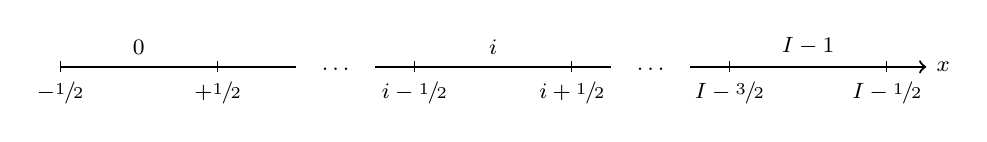
\begin{tikzpicture}
\tikzstyle{every node}=[font=\footnotesize]
\draw[thick] (0,0) -- (3,0);
\node[anchor=south] at (3.5cm,-5pt) {$\ldots$};
\draw[thick] (4,0) -- (7,0);
\node[anchor=south] at (7.5cm,-5pt) {$\ldots$};
\draw[thick,->] (8,0) -- (11,0) node[anchor=west] {$x$};

\draw ( 0 cm,2pt) -- ( 0 cm,-2pt) node[anchor=north] {$-\hzi$};
\node[anchor=south] at (1cm,1pt) {0};
\draw ( 2 cm,2pt) -- ( 2 cm,-2pt) node[anchor=north] {$+\hzi$};

\draw ( 4.5 cm,2pt) -- ( 4.5 cm,-2pt) node[anchor=north] {$i-\hzi$};
\node[anchor=south] at (5.5cm,1pt) {$i$};
\draw ( 6.5 cm,2pt) -- ( 6.5 cm,-2pt) node[anchor=north] {$i+\hzi$};

\draw ( 8.5 cm,2pt) -- ( 8.5 cm,-2pt) node[anchor=north] {$I-\sfrac{3}{2}$};
\node[anchor=south] at (9.5cm,1pt) {$I-1$};
\draw ( 10.5 cm,2pt) -- ( 10.5 cm,-2pt) node[anchor=north] {$I-\hzi$};
\end{tikzpicture}

  \caption{Notation of the one-dimensional mesh.}
  \label{fig:mesh1D}
\end{figure}

The partial currents in the case of isotropic scattering are calculated using the following expressions derived from the integral neutron transport equation~\cite{Tomatis-2011,Tomatis-2019,Gross-2020}:
\begin{subequations}
  \label{eq:par-curr-calc}
  \begin{equation}
    \label{eq:par-curr-calc-plus}
    \begin{split}
      \jp_{i+\hzi,g} &=  \frac{1}{2}
        E_3[\mcL_g(x_{-\hzi},x_{i+\hzi})] \phi_{x_{-\hzi},g} \\
        & + \frac{1}{2}\sum\limits_{j=0}^i \frac{q_{j,g}}{\sigma_{j,g}}
            \left\{ E_3\left[ \mcL_g(x_{j+\hzi},x_{i+\hzi}) \right]
                  - E_3\left[ \mcL_g(x_{j-\hzi},x_{i+\hzi}) \right]
            \right\}
    \end{split}
  \end{equation}
  %
  \begin{equation}
    \begin{split}
      \label{eq:par-curr-calc-minus}
      \jm_{i+\hzi,g} &=  \frac{1}{2}
        E_3[\mcL_g(x_{i+\hzi},x_{I-\hzi})] \phi_{x_{I-\hzi},g} \\
        & + \frac{1}{2}\sum\limits_{j=i+1}^{I-1} \frac{q_{j,g}}{\sigma_{j,g}}
            \left\{ E_3\left[ \mcL_g(x_{i+\hzi},x_{j-\hzi}) \right]
                  - E_3\left[ \mcL_g(x_{i+\hzi},x_{j+\hzi}) \right]
            \right\},
    \end{split}
  \end{equation}
where $\mcL_g(x',x)\equiv \int_{x'}^{x} \sigma_g(x'')dx''$ is the optical length. The net current is $J _{i+\hzi,g} = \jp _{i+\hzi,g} - \jm _{i+\hzi,g}$, $\forall i$. Only the zeroth moment of the angular flux, that is the scalar flux yet occurring after its expansion in angle on spherical harmonics, is used at the boundary to include the contribution of possible incoming currents. \eqs{eq:par-curr-calc} are expected to yield more accurate estimates of the currents even when using a flux distribution obtained from diffusion theory. This is the main assumption of the Ronen Method.
\end{subequations}
% \daniele{In case additional space will be needed, it will be possible to write \eqs{eq:par-curr-calc} in a condensed form by using $\pm$.}

% ------------------------------------------
\subsection{CMFD Implementation}
\label{sec:RM-CMFD}

In classic CMFD implementation, the term $\delta J_{i+\hzi,g}$ is added to the diffusion current $\jD_{i+\hzi,g}$ in order to reproduce the net current $J_{i+\hzi,g}$ used in \eq{eq:balance}. Currents are only computed on the surface elements of a coarse mesh in space to save memory and runtime \cite{Smith-1983}. Besides, the net current can be determined from some other expression which is physically or numerically more accurate. Therefore, this new term acts as a correction for the diffusion current. The diffusion current is generally approximated by discretizing Fick's law, and by finite differences, according to
\begin{equation}
  \label{eq:JD}
  \jD_{i+\hzi,g} \cong - D_{i+\hzi,g}
    \frac{\phi_{i+1,g} - \phi_{i,g}}{(\Delta_{i+1} + \Delta_i)/2},
\end{equation}
where the diffusion coefficient at the interface is volume-averaged as
\begin{equation}
  \label{eq:Ds}
  D_{i+\hzi,g} = \frac{\Delta_i D_{i,g} + \Delta_{i+1} D_{i+1,g}}
{\Delta_i + \Delta_{i+1}}.
\end{equation}
%
About the RM, more accurate estimates of the net current come from the integral expressions of \eqs{eq:par-curr-calc}, still using the scalar flux in the emission source $q_{i,g}$. In linearly anisotropic problems, the net current can also be considered to compute the source.

Once the diffusion currents and the net currents by integral transport are calculated using the most recent flux values, the correction terms can be obtained on the cell interfaces. The discretized form of the terms $\delta J_{i+\hzi,g}$ reproduce a centered drift-advection term to avoid possible indeterminate division by zeros in case of flat flux~\cite{Smith-1983,Tomatis-2011}:
\begin{equation}
  \label{eq:dJ}
  \delta J_{i+\hzi,g} = -\delta D_{i+\hzi,g}
    \frac{\phi_{i+1,g} + \phi_{i,g}}{(\Delta_{i+1} + \Delta_i)/2} =
  J_{i+\hzi,g} - \jD_{i+\hzi,g},
\end{equation}
for $i = 0, \ldots, I-2$. The division by the spatial differences can be removed because the definition of $\delta D$ is arbitrary. By retrieving the net current from \eq{eq:dJ} and substitution in \eq{eq:balance} with the source from \eq{eq:qsrc} yields the CMFD balance equation. Finally, using Eqs.~\eqref{eq:JD}, \eqref{eq:dJ} and rearranging, the flux follows by solving a system of linear equations:
%
% Daniele: the signs at superscript are not valid here. This is removed to get shorter text. A sentence is added to the previous paragraph to introduce implicitly the eqn to solove.
%
%The CMFD, eigenvalue balance equation are 
%\begin{equation}
%  \label{eq:CMFD-diff}
%  \begin{gathered}
%  J^+_{D,i+\hzi,g} + \delj^+_{i+\hzi,g} - J^-_{D,i-\hzi,g} - \delj^-_{i-\hzi,g} + \sigma_{i,g}\phi_{i,g}=\\
%  \frac{\chi_g}{\keff}\sum\limits_{g'=1}^G\nu\sigma_{f,i,g'}\phi_{i,g'} + \sum\limits_{g'=1}^G\sigma_{s,i,g\leftarrow g'}\phi_{i,g'}.
%  \end{gathered}
%\end{equation}
%Using Eqs.~\eqref{eq:JD}, \eqref{eq:dJ}, and rearranging, yields
\begin{equation}
  \label{eq:CMFD-diff-rearranged}
  \begin{split}
  \left( \frac{-D_{i-\hzi,g} + \dd_{i-\hzi,g}}{\dx_{i-1} + \dx_i}\right) &\phi_{i-1,g} \\
  + \left(\frac{D_{i+\hzi,g} - \dd_{i+\hzi,g}}{\dx_{i+1} + \dx_i} + \frac{D_{i-\hzi,g} + \dd_{i-\hzi,g}}{\dx_i + \dx_{i-1}} + \frac{\sigma_{i,g}}{2}\right) &\phi_{i,g} \\
  + \left( \frac{-D_{i+\hzi,g} - \dd_{i+\hzi,g}}{\dx_{i+1} + \dx_i} \right) &\phi_{i+1,g} = \frac{1}{2}q_{i,g},
  \end{split}
\end{equation}
for $0 < i < I-1$.

Boundary conditions applies on the diffusion current as usual by means of an extrapolated length $\zeta$, \ie{} $\zeta \jD \cong D \phi$. The constant $\zeta$ can follow from Mark or Marshak approximations, or others derived again from transport theory \cite{meghreblian1960reactor}. About the correction terms instead, it is simply $\delta J = -\delta D \phi$ with the boundary flux approximated at first order by the cell-averaged value. The introduction of these closures in the equations for $i=0$ and $i=I-1$ is straightforward.

% ------------------------------------------
\subsection{pCMFD Implementation}
\label{sec:RM-pCMFD}

The CMFD introduces in the numerical scheme a free parameter per cell surface through the correction term to adjust the diffusive solution locally. Since separate calculations of the partial currents are possible, two free parameters could be used in the discretized form of the diffusion equation. This idea leads to the development of the pCMFD scheme \cite{cho2003comparison}.

Two corrective terms are then introduced: $J = \jp - \jm = \jD + \delta J^+ + \delta J^-$. An upwind definition with respect to the direction of flight of neutrons is used for the corrections~\cite{Jarrett-2016,Zhu-2016}:
\begin{equation}
  \label{eq:CCF-sub}
  \delta \jp _{i+\hzi} = -\delta D^+ _{i+\hzi} \phi_i
  \quad \text{and} \quad
  \delta \jm _{i+\hzi} = -\delta D^- _{i+\hzi} \phi_{i+1}.
\end{equation}
It can be noted that the signs before the correction terms are arbitrary, with no need to follow a specific physical meaning. 
%
% Daniele: the signs used for the \pm J corrections is not so important because
% of the arbitrarity of the corrections themselves. But whatever the choice
% has been made, the implementation must stick closely with it.
%
The current by diffusion is distributed on the partial currents in equal parts in order to compute the new corrective coefficients $\delta D^{\pm}$,
\begin{subequations}
  \label{eq:delta-D-pCMFD}
  \begin{align}
    J^+_{i+\hzi} - \frac{1}{2}\jD_{i+\hzi} &= -\delta D^+_{i+\hzi} \phi_i, \label{eq:delta-D-pCMFDp}\\
    J^-_{i+\hzi} + \frac{1}{2}\jD_{i+\hzi} &= +\delta D^-_{i+\hzi} \phi_{i+1}, \label{eq:delta-D-pCMFDm}\\
    J^\pm_{i+\hzi} = \pm \frac{1}{2}\jD_{i+\hzi}& \mp \delta D^{\pm} _{i+\hzi} \phi_{i+(1\mp 1)/2}\label{eq:delta-D-pCMFDpm},
  \end{align}
\end{subequations}
still for $i=0, \ldots, I-2$.
% -----------------------------------------------------------------------------
%
% Daniele: the following proposition has shown to be inconsistent.
%
% Thanks to P$_1$ diffusion theory, the partial currents at any point $x$ of the slab are approximated as
% \begin{equation}
% \label{eq:partial-current}
% \jpm(x) \cong \frac{\phi(x)}{4} \pm \frac{J (x)}{2},
% \end{equation}
% still verifying the expression for the net current $J = J^+ - J^-$. \eq{eq:partial-current} suggests introducing two different correction terms at each cell interface depending on the sign of the partial currents
% \begin{equation}
%   \label{eq:PCCF}
%   \jpm _{i+\hzi} = \frac{1}{4} \phi_{i+\hzi} \pm \frac{1}{2}
%     \left(\jD_{i+\hzi} + \delta \jpm_{i+\hzi}\right),
% \end{equation}
% and they must fulfill again the net current $J = \jD + (\delta \jp + \delta \jm)/2$. An upwind definition with the respect to the direction of flight of neutrons is~\cite{Jarrett-2016,Zhu-2016}
% \begin{equation}
% \label{eq:CCF-sub}
% \delta \jp _{i+\hzi} = -2\delta D^+ _{i+\hzi} \phi_i
% \quad \text{and} \quad
% \delta \jm _{i+\hzi} = -2\delta D^- _{i+\hzi} \phi_{i+1}.
% \end{equation}
% %
% Solving for the partial current correction factors gives
% \begin{equation}
%   \label{eq:ccfsss1}
%   \delta D^+ _{i+\hzi} = \frac{\frac{1}{4}\phi_{i+\hzi}
%   	+ \frac{1}{2}\jD _{i+\hzi} - \jp _{i+\hzi}}{\phi_i}
%   \quad \text{and} \quad
%   \delta D^- _{i+\hzi} = \frac{-\frac{1}{4}\phi_{i+\hzi}
%   	+ \frac{1}{2}\jD _{i+\hzi} + \jm _{i+\hzi}}{\phi_{i+1}},
%   \end{equation}
% where the flux at the interface can be simply volume-averaged too, see~\eq{eq:Ds} for instance.
% -----------------------------------------------------------------------------
%
% Daniele: removed to get shorter text and avoid repetitions
%
%The descretized form of the diffusion equations, with pCMFD implementations, is
%\begin{equation}
%  \label{eq:pCMFD-diff1}
%  \begin{gathered}
%  J_{D,i+\hzi,g}^+ +\left( \delj_{i+\hzi,g}^+ - \delj_{i+\hzi,g}^- \right) - J_{D,i-\hzi,g}^+
%  + \left( + \delj_{i-\hzi,g}^+ - \delj_{i-\hzi,g}^- \right) \\ + \sigma_{i,g}\phi_{i,g} = q_{i,g},
%  \end{gathered}
%\end{equation}
%where
%\begin{equation}
%  \label{eq:q}
%  q_{i,g} = \frac{\chi_g}{\keff}\sum\limits^G_{g'=1}\nu\sigma_{f,g'}\phi_{i,g'} + \sum\limits_{g'=1}^G \sigma_{s,i,0,g\leftarrow g'}\phi_{i,g'}.
%\end{equation}
The same substitutions indicated in section \ref{sec:RM-CMFD} lead to the pCMFD balance equation, where after introducing Eqs. \ref{eq:JD} and \ref{eq:CCF-sub} for the currents it is in the $i$-th cell
%\begin{equation}
%  \label{eq:pCMFD-diff2}
%  \begin{split}
%  -2D_{i+\hzi}\frac{\phi_{i+1,g} - \phi_{i,g}}{\dx_{i+1}+\dx_{i}} &+\left( \dd^+_{i+\hzi,g}\phi_{i,g}  - \dd^-_{i+\hzi,g }\phi_{i+1,g}\right)
%  +2D_{i-\hzi}\frac{\phi_{i,g} - \phi_{i-1,g}}{\dx_{i}+\dx_{i-1}} \\ 
%  &- \left( \dd^+_{i-\hzi,g}\phi_{i-1,g} -\dd^-_{i-\hzi,g}\phi_{i,g}\right) +\sigma_{i,g}\phi_{i,g} = q_{i,g}.
%  \end{split}
%\end{equation}
\begin{equation}
  \label{eq:pCMFD-rearrange}
  \begin{split}
  \left(-\tild_{i-\hzi,g}+\dd^+_{i-\hzi,g}\right)&\phi_{i-1,g} \\
  + \left( \tild_{i+\hzi,g} - \dd^+_{i+\hzi,g} + \tild_{i-\hzi,g} + \dd^-_{i-\hzi,g} + \sigma_{i,g}\right)&\phi_{i,g} \\
  + \left( -\tild_{i+\hzi,g} - \dd^-_{i+\hzi,g}\right)&\phi_{i+1,g} = q_{i,g},
  \end{split}
\end{equation}
with $\tild_{i+\hzi,g} = \left. 2D_{i+\hzi,g} \middle/ (\dx_{i+1}+\dx_{i})\right.$. The diffusion current is not halved at the boundary, using only \eq{eq:delta-D-pCMFDm} or \eq{eq:delta-D-pCMFDp} at the left and at the right boundaries, respectively. Indeed, the implementation of CMFD can be upgraded to support the pCMFD scheme with minimal changes.

In a weakly absorbing medium and several mean free paths away from the boundary or a strong absorber, all correction factors $\delta D^\pm$ are expected to vanish and the net current must be fully reproduced by the diffusion current. Of course, this must be verified by the classic CMFD scheme too.

% ------------------------------------------
\section{Results}
\label{sec:res}
Two test cases are shown in this section. The first is a one-dimensional (1-D) homogeneous plane, representing a typical fuel assembly~\cite{Tomatis-2011}. The second benchmark include three different cores, which are 1-D representation of a Boiling Water Reactor (BWR) configuration~\cite{Rahnema-1997}. Both test cases are calculated and compared by two-group nodal diffusion code (denoted as $D_0$) and the Ronen method (with the implementation of CMFD and pCMFD), and are verified against a discrete ordinates S$_N$ code, with N=16. For all test cases, isotropic scattering are considered. Therefore, the diffusion coefficients for the homogeneous case, calculated by $D_g = (3\sigma_{tr,g})^{-1} = (3\sigma_g)^{-1}$. Void boundary conditions, which are implemented within the diffusion solver, in terms of extrapolated distance for each energy group, and calculated by $d_{ext,g} = 2.13 D_g$. For sake of clarity, the fast and thermal energy groups are denoted by 1 and 2, respectively.

\subsection{Homogeneous case}
\label{sec:homog}
Considering a bare slab of width 21.5 cm, representing a Pressurized Water Reactor (PWR) fuel assembly, homogenized into two energy groups with corresponding cross sections, which are shown in Table~\ref{tab:xs_hom}. Calculations were performed with $I=400$ (No. of cells).

\begin{table}[!htbp]
	\centering
	\caption{Two-group macroscopic cross sections [cm$^{-1}$] of the homogeneous case~\cite{Tomatis-2011}.}
	\label{tab:xs_hom}
	\begin{tabular}{cccccc}
		Group $g$ &  $\sigma_{g}$ & \multicolumn{2}{c}{$\sigma_{s,0,g\leftarrow g'}$} & $\chi_g$ & $\nu\sigma_{f,g}$ \\[3mm]
		1 & 5.3115$\times$10$^{-1}$ & 5.04664$\times$10$^{-1}$ & 2.03884$\times$10$^{-3}$ & 1 & 7.15848$\times$10$^{-3}$ \\
		2 & 1.30058$\times$10$^{0}$& 1.62955$\times$10$^{-2}$ & 1.19134$\times$10$^{0}$	& 0 & 1.41284$\times$10$^{-1}$ \\
	\end{tabular}
\end{table}

Fig.~\ref{fig:slab-fluxes} shows the fast and thermal fluxes calculated by diffusion, CMFD, pCMFD and S$_{16}$ of the left half slab. The abscissa's values are the group-dependent neutron mean free path (mfp) $\tau$. One or two mpf's from the boundary towards the center of the slab are enough for diffusion, to match well the reference S$_16$ results. On the other hand, closer to the boundary, the Ronen method shows better results. 

\begin{figure}[!htbp]
	\centering
	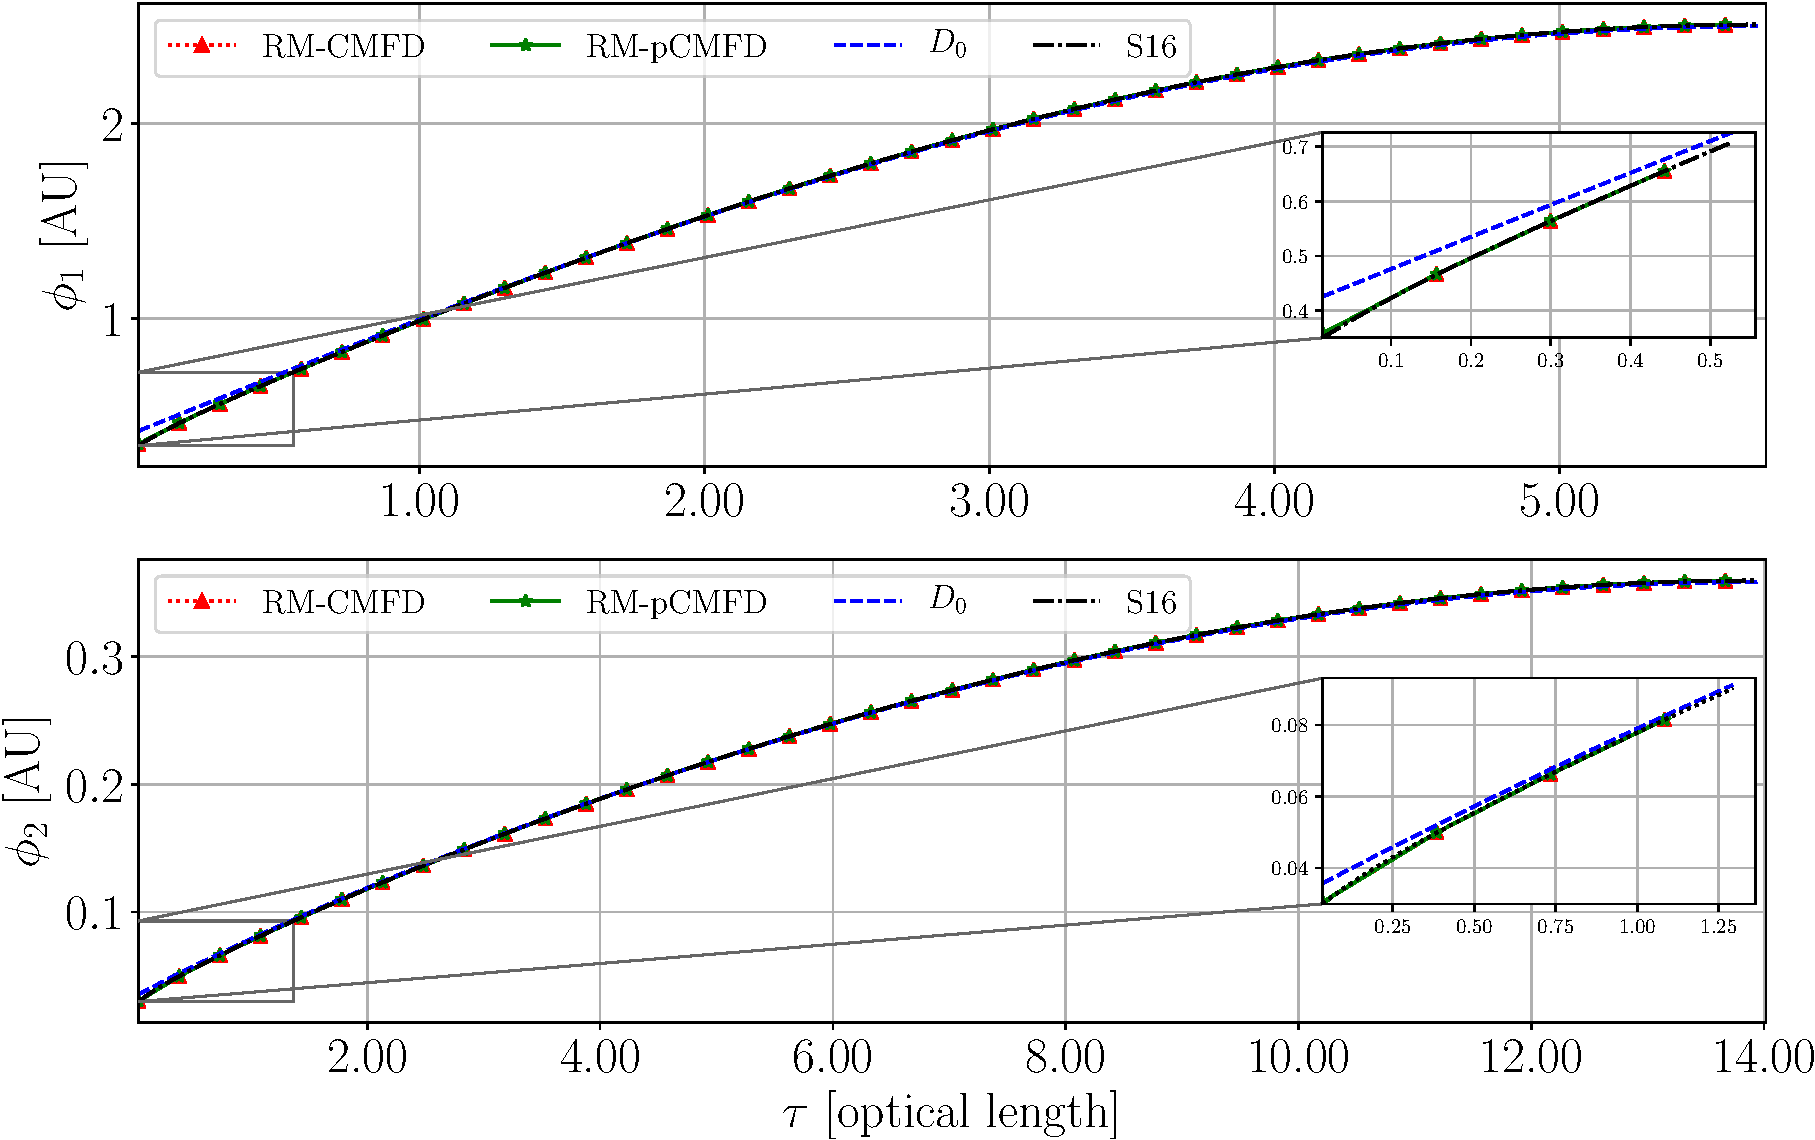
\includegraphics[width=0.9\linewidth]{Tomatis2011_flx_I400_RMitr250.pdf}
	\caption{Comparison of the fluxes as calculated by the reference S$_N$, RM-CMFD - RM-pCMFD codes, and a standard multigroup diffusion without RM correction ($D_0$). The insets show a zoom-in of the fluxes near the boundary. Results shown here after 250 Ronen iterations and 400 cells.}
	\label{fig:slab-fluxes}		
\end{figure}

In Fig~\ref{fig:flx_err_homg}, the flux deviation (calculated by $\Delta \phi = \left[\left(\phirm-\phiref\right)/\phiref\right]\times 100$) at the first 40 cells of the left slab has approximately $\sim 20\%$ difference between diffusion and RM calculations. The difference observed closer to the boundary, due to the fact that the major transport effect occur near the boundary of the homogeneous slab. 

\begin{figure}[!hbtp]
	\centering
	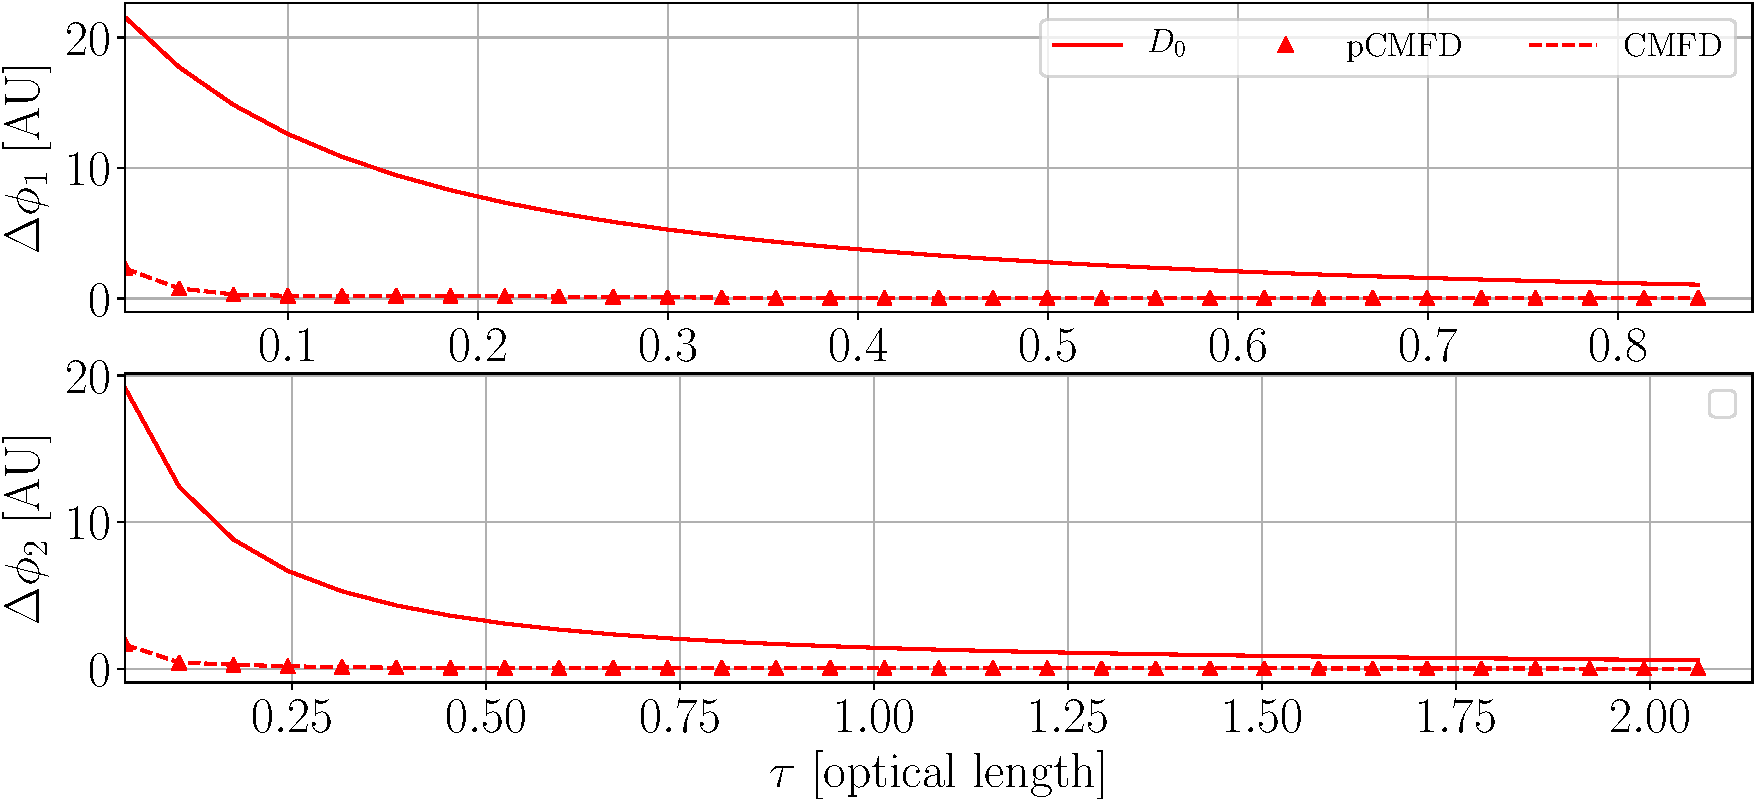
\includegraphics[width=0.9\linewidth]{Tomatis2011_flx_err_I400_RMitr250.pdf}
	\caption{The spatial flux deviation of the RM-CMFD and RM-pCMFD iterations with respect to the reference S$_{16}$ solution for the left half slab.}
	\label{fig:flx_err_homg}
\end{figure}

A comparison of the flux deviation, calculated by the two implementations of the RM, within the left-most (I=0) cell is shown in Fig.~\ref{fig:slab-fluxes-dev-LB}. The deviation of CMFD and pCMFD has very close trend along the 250 iterations, reaching approximately $\sim 2\%$ compared to the reference solution.

\begin{figure}[!htbp]
	\centering
	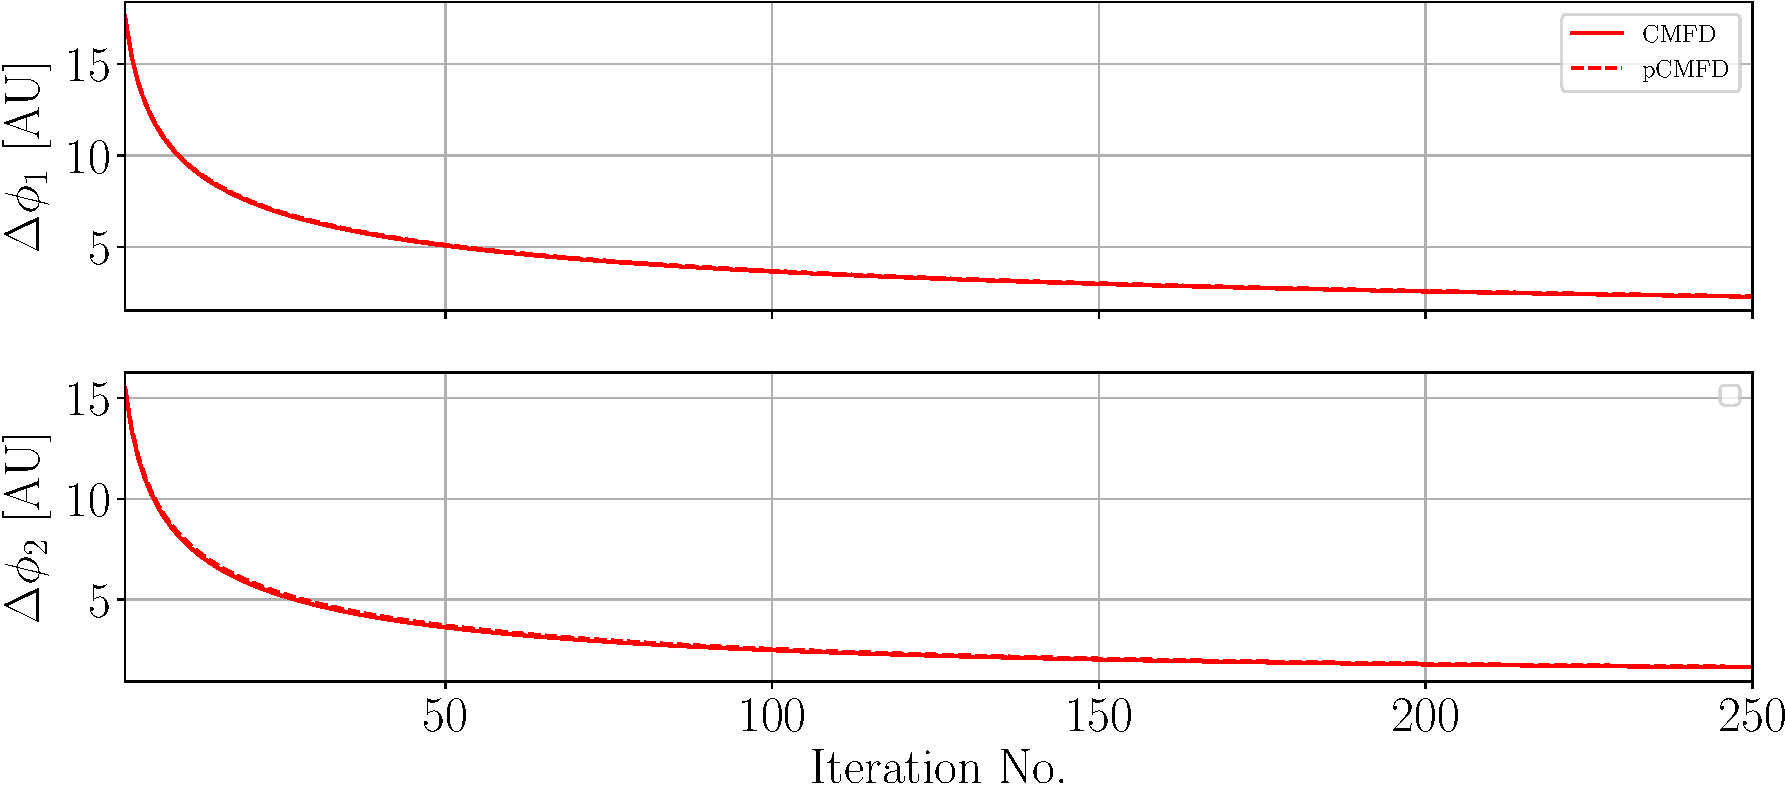
\includegraphics[width=0.9\linewidth]{Tomatis2011_flx_err_LB_I400_RMitr250.pdf}
	\caption{Deviation of the fluxes at the left-most cell, calculated by RM-CMFD and RM-pCMFD codes, with respect to the reference solution after 250 Ronen iterations.}
	\label{fig:slab-fluxes-dev-LB}
\end{figure}


In Fig~\ref{fig:rho_homg}, the behavior of the eigenvalue difference $\Delta\keff$ in pcm, along RM iterations are represented, and calculated by $\Delta\keff = \left(\keff^{-1}-\kref^{-1}\right)\times 10^5$ pcm. The value of the eigenvalues reported by the reference S$_{16}$ solution is  $\kref = 0.74441$,  and by diffusion calculation $\keff = 0.74133$, which gives the value $\Delta\keff \approx 558$ pcm. One RM iteration resulting in tens of pcm, but CMFD perform well than pCMFD at the very first few iterations. After a steep decline of $\Delta\keff$, achieving by 10 iterations, both numerical implementations converging at the same rate, with a typical linear equation, approximated by $\Delta\keff \approx 4.545\cdot 10^-7 \times (\#\text{it}) + 0.744363$, it stands for iteration.

\begin{figure}[!htbp]
	\centering
	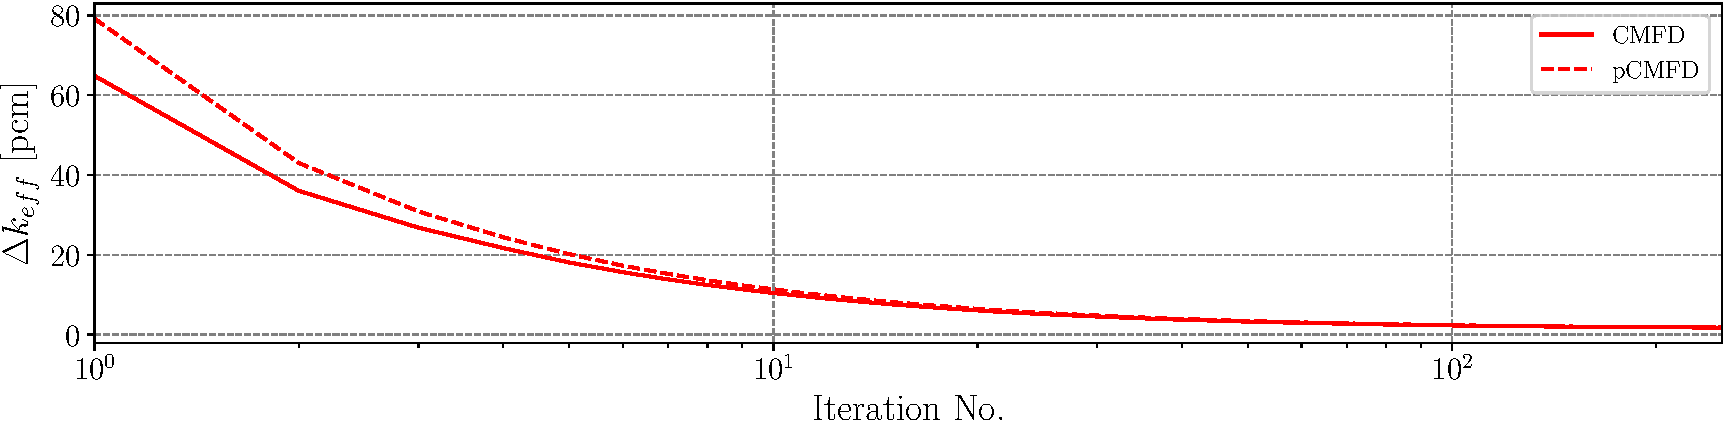
\includegraphics[width=0.9\linewidth]{Tomatis2011_dk_I400_RMitr250.pdf}	
	\caption{Convergence of the reactivity along 250 Ronen iterations, with respect to S$_N$.}
	\label{fig:rho_homg}
\end{figure}

The correction factors of CMFD and pCMFD (denoted by $\dd$, $dD^{\pm}$, respectively) are shown in Fig~\ref{fig:slab-RM-dD}. The correction factor $\dd$ calculated by CMFD, are equal to zero within the slab, but have different behavior closer to the boundaries. On the other hand, the current corrections are about $\dd^{\pm} \sim \mp 1/4$ at the center of the slab, and have particular behavior close to the boundaries. The flat steady values of the factors at the center of the slab (or few mfp's away from the boundary) can be explained by the following simple relations.  within the definition of the current $J(x,\mu)^\pm$ as follows
\begin{equation}
\label{eq:current_def}
J^\pm(x,\mu) = \int\limits_0^{\pm 1} d\mu\,\mu\,\varphi(x,\mu)\,\,.
\end{equation}
Expanding the angular flux $\phi(x,\mu)$ by $P_1$ approximation
\begin{equation}
\label{eq:p1}
\varphi(x,\mu) = \sum\limits_{l=0}^{L=1}\frac{2l+1}{2}P_l(\mu)\varphi_l(x) = \frac{1}{2}\varphi_0(x) + \frac{3}{2}\mu\varphi_1(x)\,\,,
\end{equation}
Substituing into Eq.~\ref{eq:current_def}, and integrating
\begin{equation}
	\begin{split}
		\label{eq:current_p1}
		J^\pm(x,\mu) &= \int\limits_0^{\pm 1} d\mu\mu\left[\frac{1}{2}\varphi_0(x) + \frac{3}{2}\mu\varphi_1(x)\right] \\
		J^\pm(x) &= \frac{1}{4}\phi_0(x) \pm \frac{1}{2}\varphi_1(x)\,\,.
	\end{split}
\end{equation}
The descretized form is
\begin{equation}
\label{eq:curent_p1_i}
J^\pm_{i+\hzi} = \frac{1}{4}\phi_{0,i+\hzi} \pm \frac{1}{2}J^{\pm}_{i+\hzi}\,\,.
\end{equation}
The first moment of the flux ($\varphi_1$) is the current $J$. Assuming that Fick's law is accurate, i.e. several mfp's away from significant gradients (boundary in a homogeneous slab), and in weakly absorbing medium, 
by equalizing Eq.~\ref{eq:delta-D-pCMFDpm} and Eq.~\ref{eq:curent_p1_i}, rearranging and segregating the current corrections on one side of the equation, one gets
\begin{equation}
	\label{eq:dd_quarter}
	\begin{split}
	\pm \frac{1}{2}\jD_{i+\hzi} \mp \delta D^{\pm} _{i+\hzi} \phi_{0,i+(1\mp 1)/2} & = \frac{1}{4}\phi_{0,i+\hzi} \pm \frac{1}{2} J^{\pm}_{D,i+\hzi} \\
	\dd^\pm_{i+\hzi} \approx \mp \frac{1}{4}\cdot\frac{\phi_{0,i+\hzi}}{\phi_{0,i+(1\mp 1)/2}} & \approx \mp\frac{1}{4}\,\,.
	\end{split}
\end{equation}

\begin{figure}[!htbp]
	\centering
	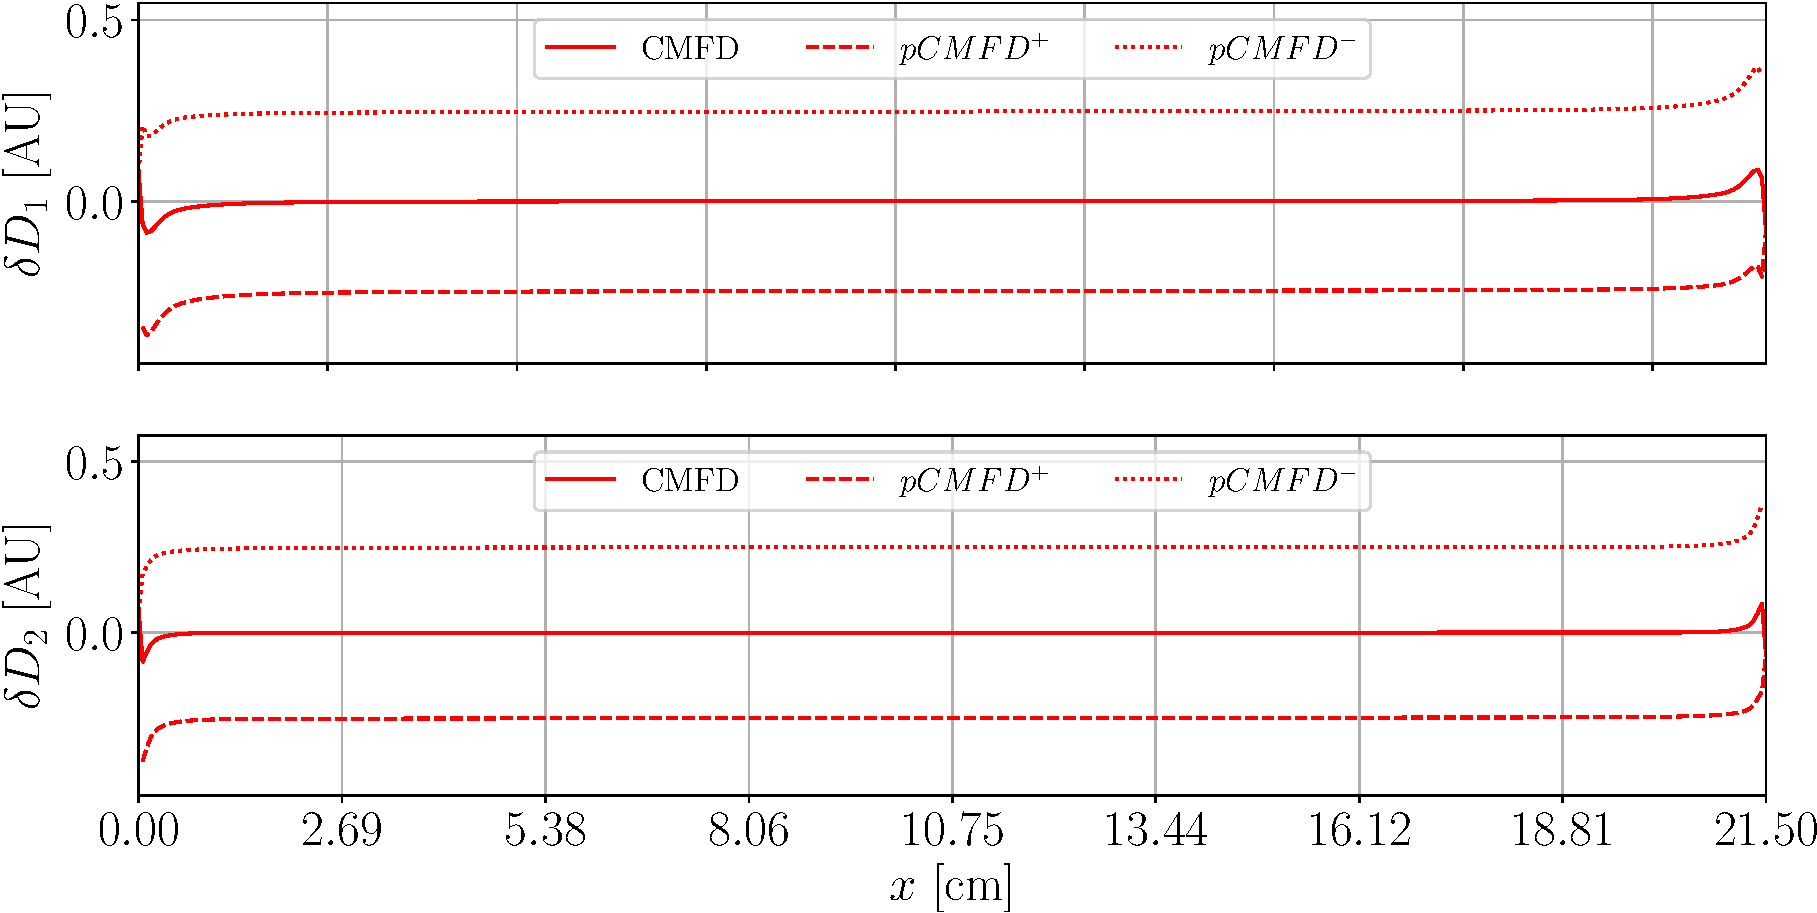
\includegraphics[width=0.9\linewidth]{Tomatis2011_dD_I400_RMitr250.pdf}
	\caption{The Ronen method correction factors ($\delta D$), calculated by CMFD code, and ($dD^{\pm}$), calculated by pCMFD code. Results shown here after 250 Ronen iterations.}
	\label{fig:slab-RM-dD}
\end{figure}

\subsection{Heterogeneous case}
\label{sec:heterog}






% ------------------------------------------
\section{Conclusions}
\label{sec:conc}

Present your summary and conclusions here.

% ------------------------------------------
%\section*{NOMENCLATURE}
%
%\begin{itemize} \itemsep1pt \parskip0pt \parsep0pt
%\item RM - Ronen Method
%\item CMFD - Coarse Mesh Finite Difference
%\item pCMFD - partial current CMFD
%\end{itemize}

%
% ------------------------------------------
%\section*{ACKNOWLEDGEMENTS}
%
%Acknowledge the help of colleagues and sources of funding, as appropriate.
%
% ------------------------------------------
% You can enter a bibliography into the document using the following format, or use the
% bibliography style file "physor.bst" found in the template directory.  You can use the bibliography style file
% by replacing the current bibliography block with:
\setlength{\baselineskip}{12pt}
\bibliographystyle{physor}
\bibliography{RM-bib}
% ------------------------------------------
%\appendix
%\gdef\thesection{APPENDIX \Alph{section}}
%\section{Sample Appendix 1}
%\label{app:a}
%If necessary, include Appendices numbered in upper case alphabetical order. This is \ref{app:a}.
%
\end{document}
